This section examines how the time paths for optimal drilling and production vary with oil prices. Using the Implicit Function Theorem, we first predict the impact of a sudden price variation on the drilling probability, which governs the optimal paths of drilling and production. We then demonstrate how the optimal drilling and production paths respond to unexpected demand shocks. We also investigate the heterogeneous impacts of unanticipated demand shocks on drilling well sites of different quality. Finally, we compute the equilibrium paths under two different scenarios for oil prices: exogenous and endogenous oil prices.


\subsection{Impacts of Unexpected Demand Shocks}
\label{C3-SubSection:Impacts-of-Unexpected-Demand-Shocks}
\afterpage{
    \begin{figure}[t!]
        \centering
        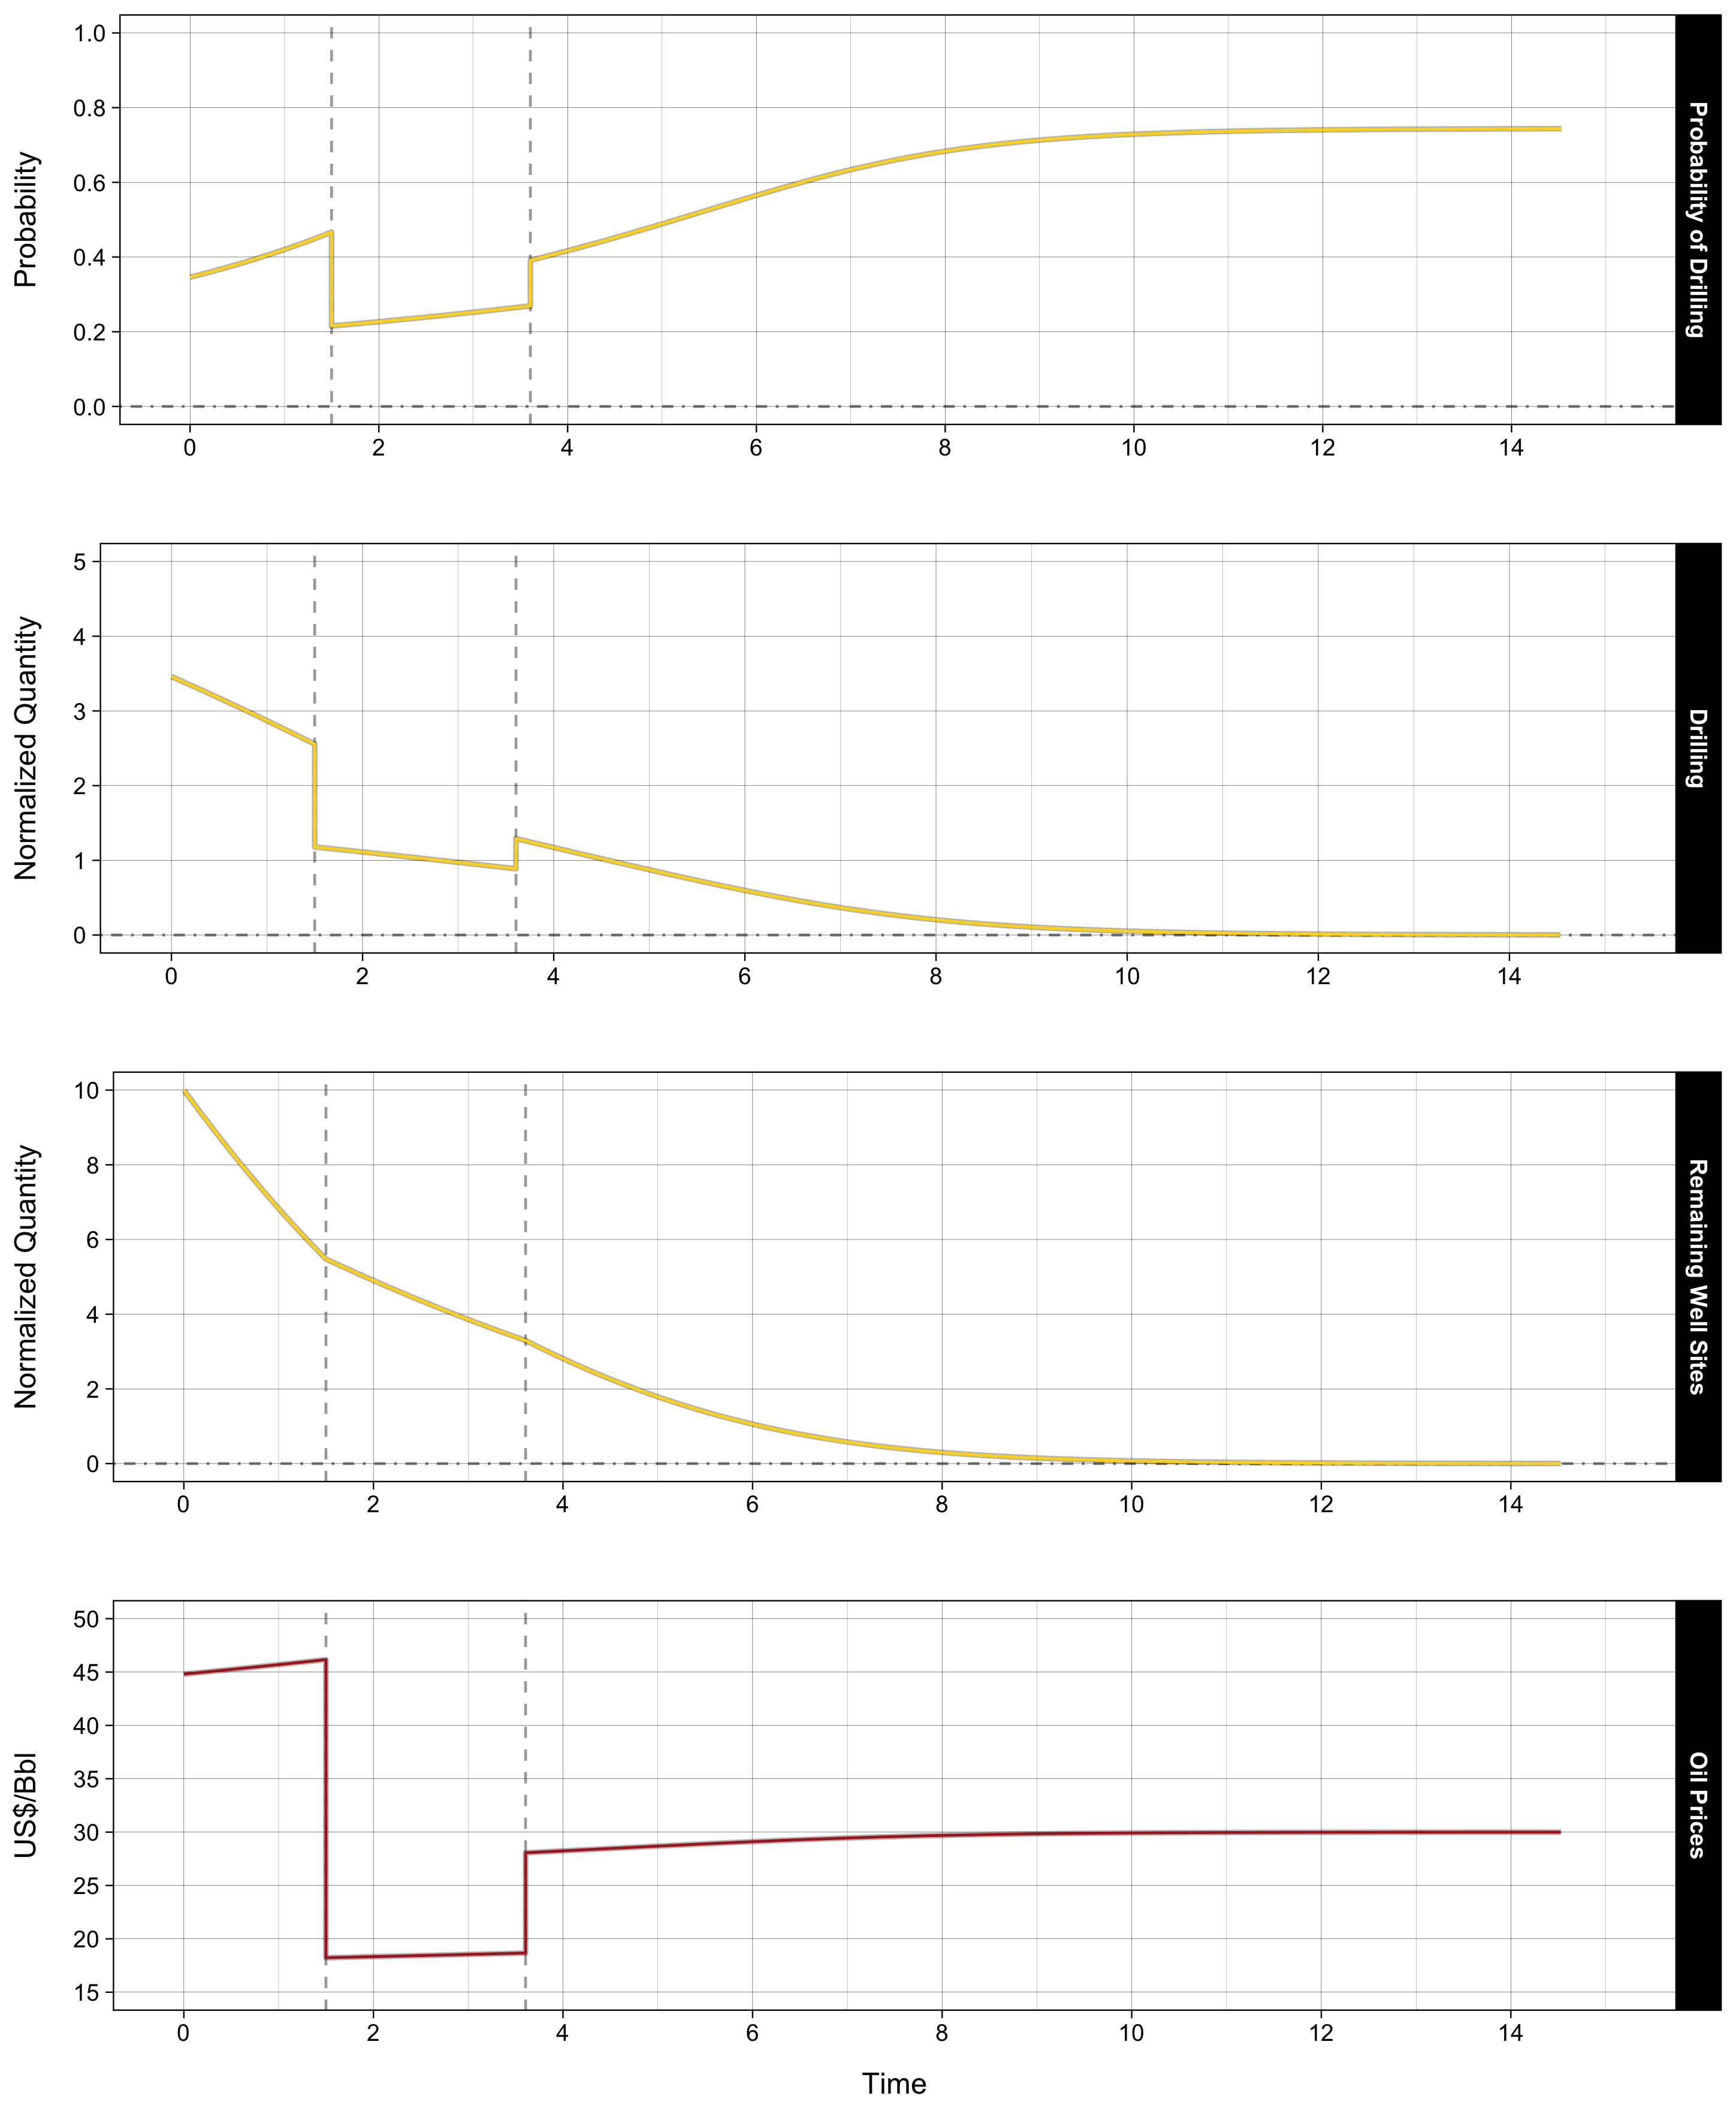
\includegraphics[scale = 0.15]{04_Chapter-3/00A_Figures/Figure_Equlibrium-Paths_Endogenous-Price.png}
        \caption{Equilibrium Paths under Unexpected Demand Shocks}
        \caption*{
            {\small
            \textit{Note}: 
            This figure shows the equilibrium paths of drilling probability, drilling, and the remaining well sites, which are obtained from a simulation for two unanticipated demand shocks. For these simulation results, we assume the identical parameter values and cost function utilized to draw the phase diagrams in Figure \ref{Figure:Phase-Diagram_Saddle-Point}.
        }}
        \label{Figure:Equilibrium-Paths-under-Unexpected-Demand-Shocks}
    \end{figure}
}
The Implicit Function Theorem (IFT) allows us to predict the impact of sudden demand shocks on the equilibrium paths for drilling and production. Applying the IFT to equation (\ref{Equation:Firms-Problem_Euler-Equation}) (i.e., the Euler equation of the firm's problem) yields
\begin{align}
    % \frac{ \ f_{ik} \ + \ \lambda_{a} \sigma \big( \gamma \ - \ \ln(1 - Pr_{k}) \big) \ }{\rho} \
    % & = \ \left\{ \psi_{i1k} \ + \ \sigma \big( \gamma \ - \ \ln(Pr_{k}) \big) \right\} \ - \ \sigma \big( \gamma \ - \ \ln(1 - Pr_{k}) \big) \\
    % \frac{1}{\rho} \frac{\partial f_{ik}}{\partial p_{k}} \ + \ \frac{\lambda_{a} \sigma}{\rho (1 - Pr_{k})} \frac{\partial Pr_{k}}{\partial p_{k}} \
    % & = \ \frac{\partial \psi_{i1k}}{\partial p_{k}} \ - \ \frac{\sigma}{Pr_{k}} \frac{\partial Pr_{k}}{\partial p_{k}} \ - \ \frac{\sigma}{1 - Pr_{k}} \frac{\partial Pr_{k}}{\partial p_{k}} \\
    % \left( \frac{\lambda_{a} \sigma}{\rho (1 - Pr_{k})} \ + \ \frac{\sigma}{Pr_{k}} \ + \ \frac{\sigma}{1 - Pr_{k}} \right) \frac{\partial Pr_{k}}{\partial p_{k}} \
    % & = \ -\frac{1}{\rho} \frac{\partial f_{ik}}{\partial p_{k}} \ + \ \frac{\partial \psi_{i1k}}{\partial p_{k}} \\
%    \frac{\partial Pr_{k}}{\partial p_{k}} \
%    & = \ \left\{ \frac{\rho Pr_{k} (1 - Pr_{k})}{\sigma (\lambda_{a} Pr_{k} + \rho)} \right\} \left( \frac{\partial \psi_{i1k}}{\partial p_{k}} \ - \ \frac{1}{\rho} \frac{\partial f_{ik}}{\partial p_{k}} \right).
    \frac{\partial Pr_{k}}{\partial p_{k}} \
    & = \ \left\{ \frac{\rho Pr_{k} (1 - Pr_{k})}{\sigma (\lambda_{a} Pr_{k} + \rho)} \right\} \frac{\partial \psi_{i1k}}{\partial p_{k}}.
\label{Equation:Equilibrium-Paths_Applying-IFT}
\end{align}
This resulting equation suggests that an unexpected positive price shock will lead to a higher drilling rate if the cost-shock-induced incremental gains from drilling are larger than those from waiting (i.e., $\partial \psi_{i1k}/\partial p_{k} - (1/\rho)(\partial f_{ik}/\partial p_{k}) > 0$).\footnote{If $Pr_{k} \in (0, 1)$, every term in the curly bracket is always positive.}
\afterpage{
    \begin{figure}[t!]
        \centering
        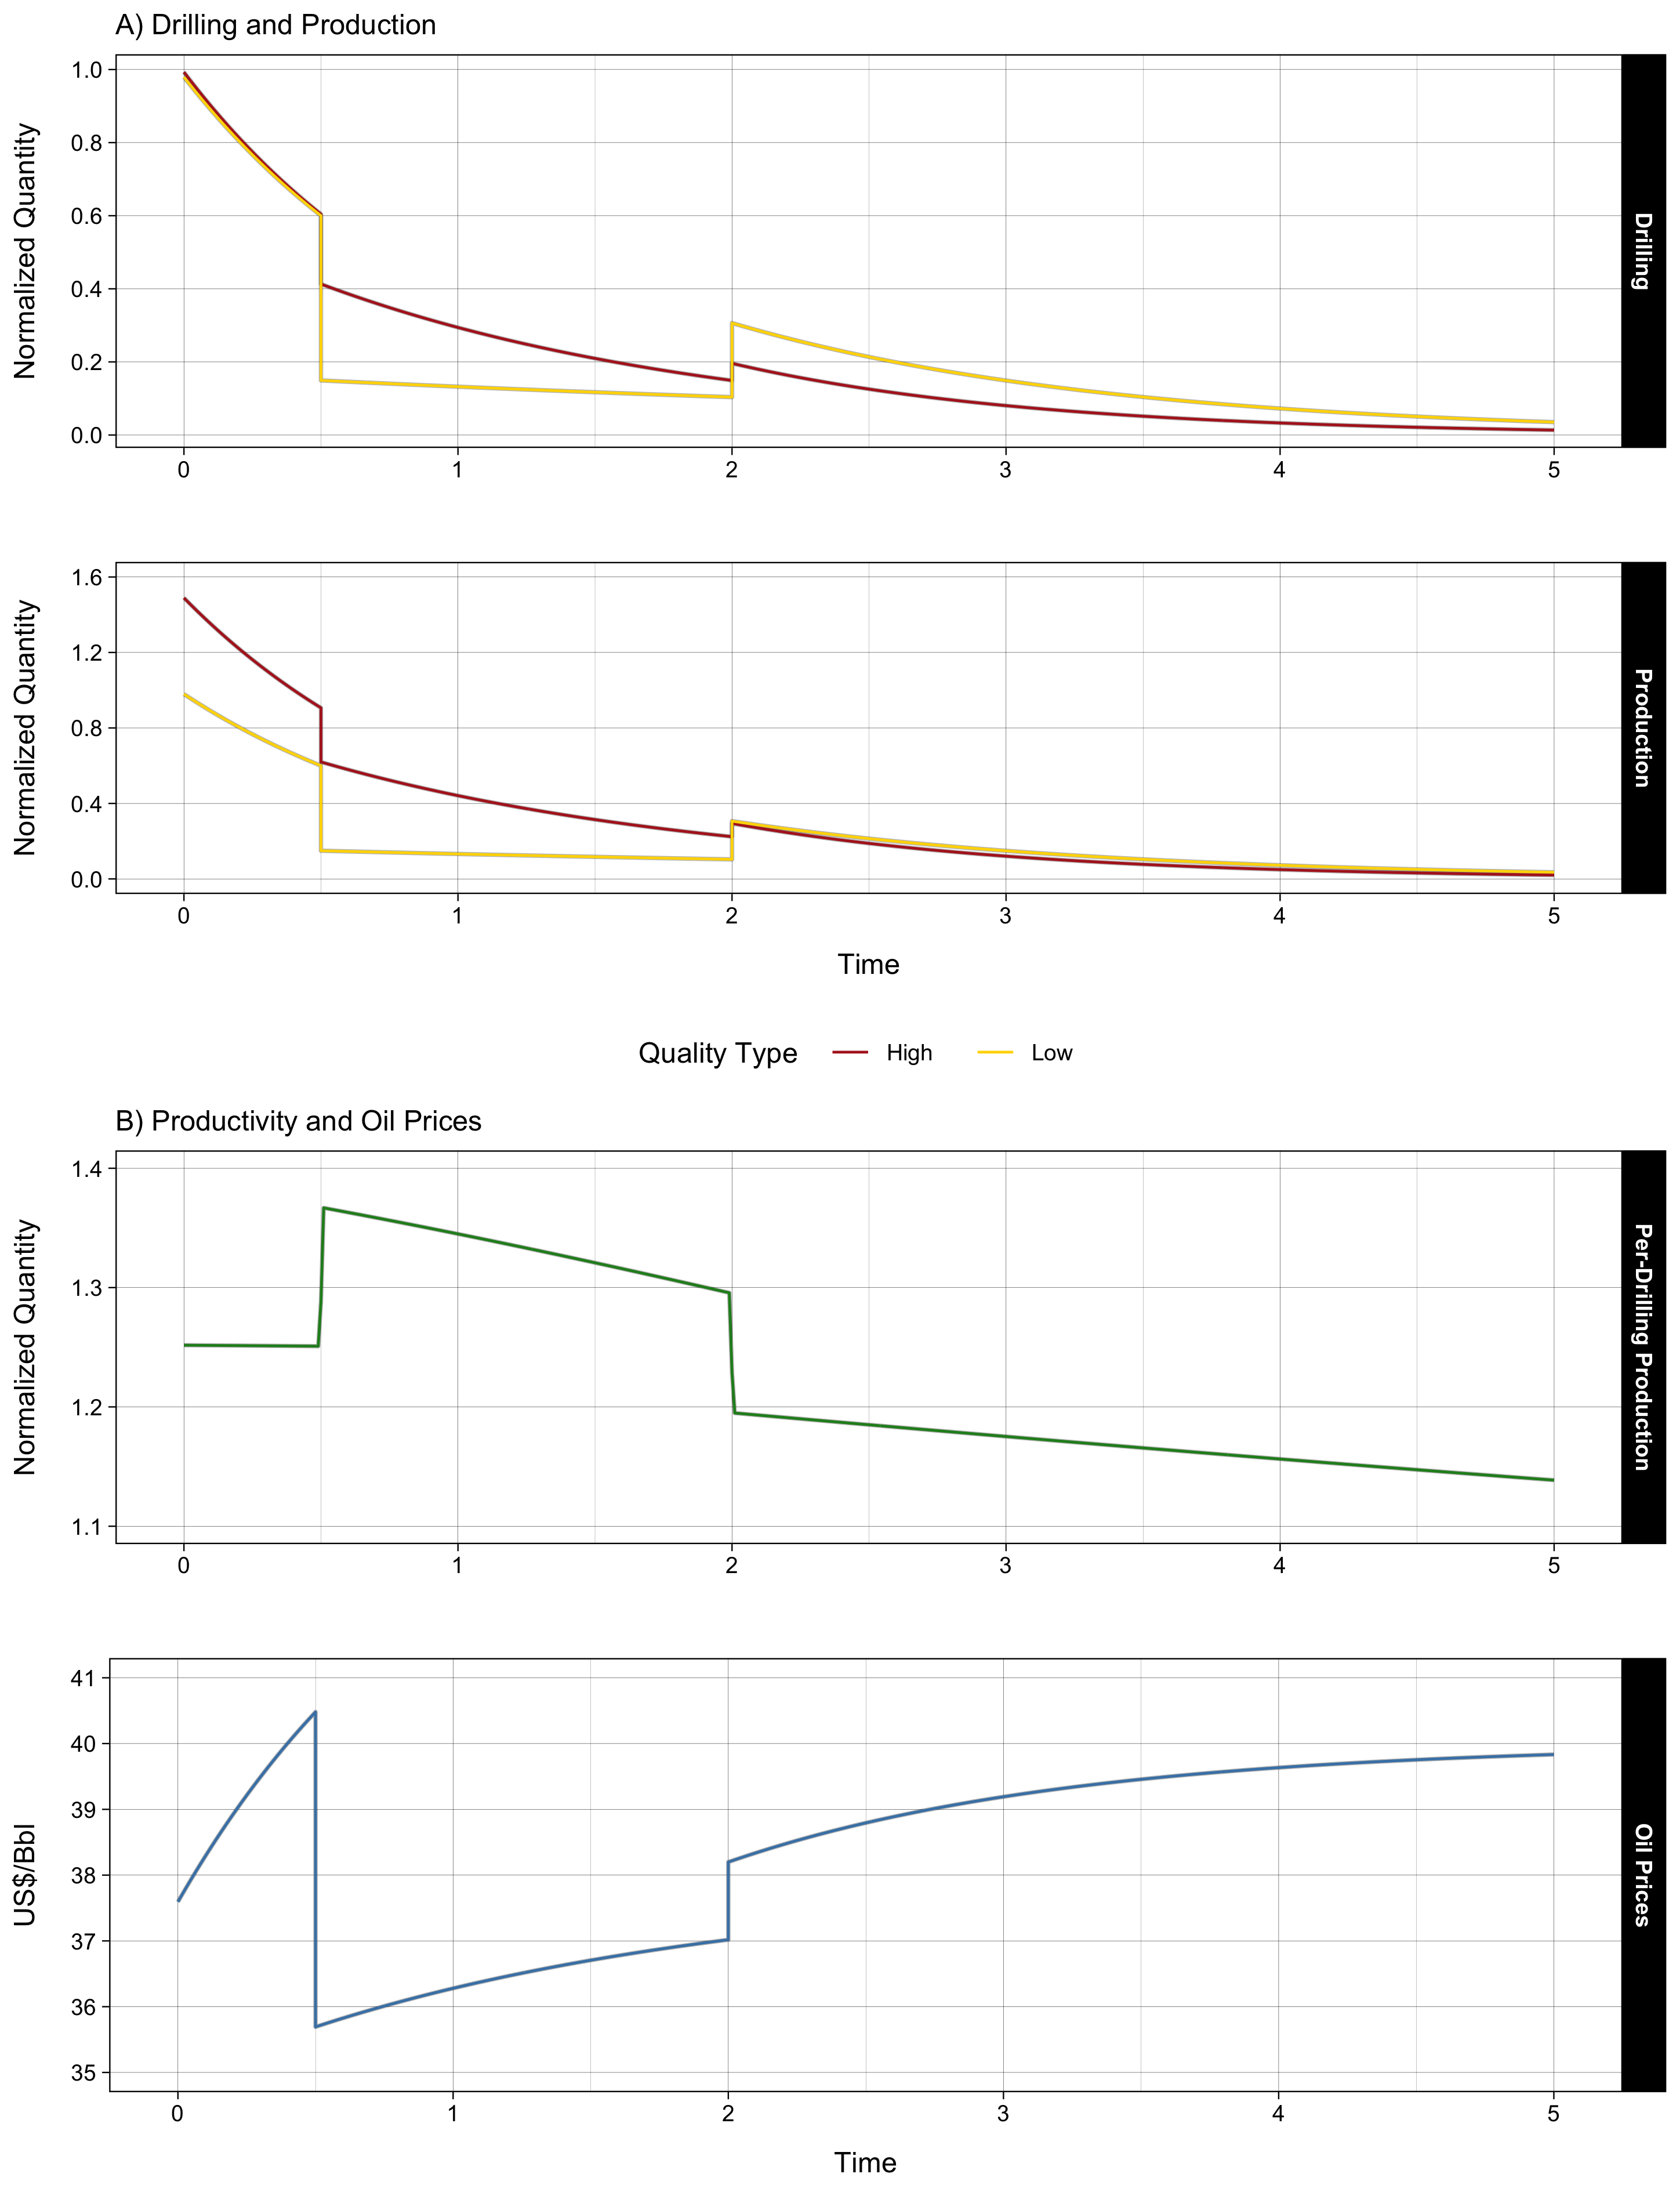
\includegraphics[scale = 0.11]{04_Chapter-3/00A_Figures/Figure_Impact-of-Demand-Shocks-on-Drilling-of-Well-Sites-with-Heterogeneous-Quality}
        \caption{Heterogeneous Impacts of Unexpected Demand Shocks on Drilling and Production}
        \caption*{
            {\small
            \textit{Note}: 
            This figure demonstrates how the firm's drilling activity at well sites of heterogeneous quality responds to unexpected demand shocks. As shown in the first panel, the drilling probability of low-quality well sites shows a higher sensitivity to the first negative demand shock. The second panel demonstrates that although the drilling probability of low-quality well locations more sensitively responds to the second positive demand shock, the probability is still lower than that of high-quality well sites. The third panel illustrates the impacts of the demand shocks on oil extraction productivity. Clearly, the first negative shock discontinuously increases per-drilling oil production due to the high sensitivity of low-quality location drilling. To the second positive demand shock, the per-drilling production showed the opposite reaction. For this simulation, we assume that a dispersion parameter of $\sigma = 1$, an interest rate of $r = 0.05$, an initial number of well sites of $R_{0}^{g} = 1$, additional well sites of $E^{g} = 0$, where $g \in \{ L, H \}$. Also, it is assumed that a flow payoff function of $f(p_{k}) = 20 - 0.5p_{t}$ and that an instantaneous payoff function of $\psi_{iak} (p_{k}, a) = [\{ g_{i}^{L} + 1.5(1 - g_{i}^{L}) \} p_{k} - 2]a$. 
        }}
        \label{Figure:Heterogeneous-Impacts-of-Unexpected-Price-Shocks-on-Equilibrium-Paths}
    \end{figure}
}

Figure \ref{Figure:Equilibrium-Paths-under-Unexpected-Demand-Shocks} depicts how the paths of drilling probability, drilling, reserves, and oil price respond to two unanticipated demand shocks.\footnote{Given parameter values utilized for this simulation, the condition for the positive relationship between drilling probability and unexpected price shocks in (\ref{Equation:Equilibrium-Paths_Applying-IFT}) (i.e., $\partial \psi_{i1k} / \partial p_{k} - (1/\rho)(\partial f_{ik} / \partial p_{k}) > 0$) holds.} The first negative demand shock causes drilling probability discontinuously decreases. Due to the reduction in drilling probability, drilling demonstrates a discontinuous decrease too. Moreover, the negative demand shock also reduces the depletion rate of the remaining well locations. As shown in the last panel in the figure, the oil price jumps down on impact after the negative demand shock, then gradually rises.\footnote{Drilling, and thus production, rapidly diminishes for a while after $t = 0$. Then, its rate of change gradually decreases, and drilling eventually converges to a lower bound. In other words, the time path of drilling has a convex profile. Because equation (\ref{Equation:Firms-Problem_Oil-Prices}) determines the oil price at time $t$, the time path for the endogenous oil price is a concave curve.} The later positive demand shock induces the opposite reactions in the equilibrium paths. 


\subsection{Heterogeneous Impacts of Unanticipated Demand Shocks on Drilling Well Sites of Different Quality}
\label{C3-SubSection:Heterogeneous-Impacts-of-Unanticipated-Demand-Shocks-on-Drilling-Well-Sites-of-Different-Quality}
To examine how the firm's drilling activity at well sites of heterogeneous quality responds to unexpected demand shocks, we suppose that a particular well location $i$ has a quality type that falls in one from the quality set $\mathcal{Q} = \{ L(ow), H(igh) \}$. Furthermore, we also assume that when the well location is not drilled yet, the choice-specific instantaneous payoff $\psi_{i \alpha k}$ takes the following functional form:
\begin{align}
    \psi_{iak}(p_{k}; \boldsymbol{\theta}_{\psi}) \
    & = \ \big\{ g_{i}^{L} \ + \ (1 - g_{i}^{L}) \alpha^{H} \big\} p_{k} \ - \ c,
\label{Equation:Firms-Problem_Instantaneous-Payoff-for-Heterogeneous-Quality}
\end{align}
where $g_{i}^{L}$ is a binary indicator with the value of one when well location $i$ is a low-quality well site and $\alpha^{H}$, which is greater than 1, is the normalized oil production from the site $i$ whose quality type is $H$.\footnote{In the formulation, we implicitly normalize the oil production from a well location to 1.} 

Figure \ref{Figure:Heterogeneous-Impacts-of-Unexpected-Price-Shocks-on-Equilibrium-Paths} illustrates the results from a simulation. As discussed in Section \ref{C3-SubSubSection:The-Role-of-Geological-Quality-in-Horizontal-Drilling}, our empirical analysis reveals that fracking firms in North Dakota more significantly reduced drilling at low-quality well sites, more than at the high-quality ones, when experiencing sharp oil price declines. The time paths for drilling and production presented in the figure clearly show that the model-predicted elasticity of drilling s greater on low-quality well sites, just as illustrated in Figure \ref{Figure:High-Sensitivity-of-Firm-Level-Low-Quality-Well-Drilling}.\footnote{The term $Pr_{k}(1 - Pr_{k})$ in equation (\ref{Equation:Equilibrium-Paths_Applying-IFT}) is a parabolic curve that goes to zero as $Pr_{k}$ approaches to zero or one and that has its maximum value at $Pr_{k} = 1/2$. These properties of the term suggest the possibility that the drilling of high-quality well sites is less responsive to a demand shock.} As demonstrated in the third panel of the figure, per-drilling production, i.e., productivity, increases discontinuously due to the negative demand shock. Consequently, as described in the fourth panel, per-drilling oil production is also improved. 


\subsection{Exogenous vs. Endogenous Oil Prices}
\label{C3-SubSection:Exogenous-vs-Endogenous-Oil-Prices}
This section examines the equilibrium path of drilling for each of the exogenous and endogenous oil prices. Endogenizing the time path of oil prices makes the probability of drilling at time $t = 0$ decrease due to the initial production (i.e., $Q_{0} > 0$). Since increasing drilling, and thus production, causes oil prices endogenously determined to fall, there would be no incentive to rapidly raise the rate of drilling. For these reasons, drilling under endogenous oil prices (denoted $D_{t}^{en}$) would be small relative to that under exogenous oil prices (denoted $D_{t}^{ex}$) for some period after $t = 0$. But at some time point, $D_{t}^{en}$ would be larger than $D_{t}^{ex}$ because of the lower level of undrilled reserves in the exogenous-price case. Figure \ref{Figure:Time-Paths-for-Drilling-and-Reserves-under-Endogenous-and-Exogenous-Oil-Prices}, which shows the time paths for drilling and the remaining reserves for each type of oil price, supports the predictions.

